\cleardoublepage
\chapter{PERANCANGAN}
\label{chap:perancangan}

\section{Arsitektur Konseptual Sistem}

Bagian ini menguraikan landasan konseptual dan fungsional dari penyesuaian alur sistem pemantauan kualitas udara melalui evaluasi terhadap karakteristik sistem berjalan serta penyusunan kerangka kerja usulan yang diorientasikan pada karakteristik pemodelan yang adaptif. {Perancangan arsitektur sistem nyata ini merupakan implementasi fisik dan perwujudan praktis dari kerangka konseptual transformasi data-ke-luaran yang telah dirumuskan secara teoretis pada Subbab \ref{subsection:kerangka_transformasi}.} Perancangan arsitektur konseptual ini bertujuan untuk memberikan gambaran mengenai aliran informasi dan logika pemrosesan data, dengan menekankan pada pergeseran fungsionalitas dari pelaporan data historis menjadi komponen analisis prediktif. Integrasi pemodelan komputasi berbasis \textit{machine learning} dalam arsitektur usulan dirancang untuk memproses karakteristik data polusi udara di Jakarta sehingga diharapkan mampu mengurangi nilai kesalahan estimasi guna membantu proses pemantauan lingkungan.

\subsection{Sistem Berjalan (\textit{Existing Sistem})}

Sistem pemantauan kualitas udara yang dikelola oleh Dinas Lingkungan Hidup Provinsi DKI Jakarta saat ini menggunakan arsitektur pemrosesan satu arah. Secara operasional, data mentah ditarik dari stasiun pemantauan, dikonversi menjadi Indeks Standar Pencemar Udara (ISPU), dan didistribusikan kepada masyarakat melalui kanal digital resmi. Alur sistem berjalan yang bersifat linear ini mencerminkan proses pengolahan data konvensional yang belum mengintegrasikan pemodelan prediktif secara otomatis.

Secara arsitektural, sistem ini beroperasi sebagai entitas penyimpan dan pelapor data historis (\textit{data logger and reporter}) yang bersifat pasif. Keterbatasan analitik prediktif menyebabkan sistem memetakan kondisi kualitas udara yang telah terjadi tanpa menyediakan estimasi nilai untuk periode mendatang. Hal ini memengaruhi kegunaan data dalam upaya penentuan langkah mitigasi dan perencanaan kebijakan perlindungan kesehatan masyarakat yang memerlukan informasi proyeksi polusi secara antisipatif.

Karakteristik pada modul pemrosesan menyebabkan data mentah belum diproses melalui rekayasa fitur secara multivariat untuk menangkap variasi atmosferik yang dinamis. Tanpa adanya modul inferensi yang memadai, sistem memproses data historis tanpa menghasilkan proyeksi nilai yang dapat digunakan oleh pemangku kepentingan. Akibatnya, sistem belum menyediakan acuan numerik mengenai proyeksi kualitas udara untuk mengantisipasi fluktuasi polutan, sebagaimana ditunjukkan pada diagram alir Gambar \ref{gambar:sistem_sebelum}.

\begin{figure}[htbp]
  \centering
  \captionsetup{justification=centering}
  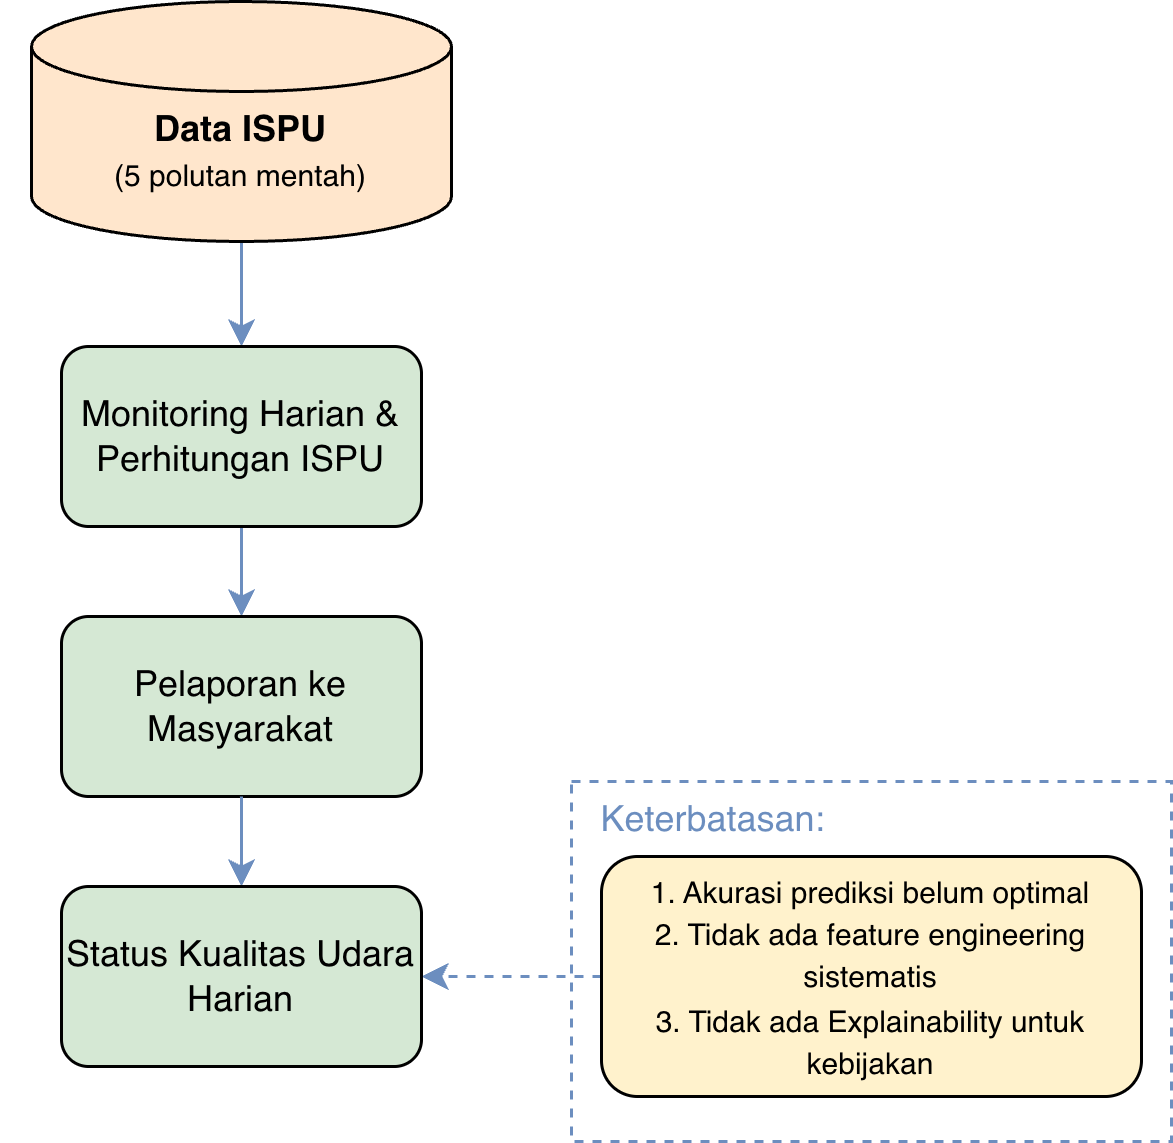
\includegraphics[width=0.4\textwidth]{images/sistem_sebelum.png}
  \caption{Diagram sistem pemantauan kualitas udara Jakarta saat ini (Sistem Berjalan)}
  \label{gambar:sistem_sebelum}
\end{figure}

\subsection{Arsitektur Usulan (\textit{Proposed Sistem})}

Untuk meminimalkan keterbatasan arsitektur yang ada, penelitian ini merancang ulang arsitektur sistem dengan menambahkan komponen pemodelan prediktif ke dalam alur informasi secara terintegrasi. Dengan mengadopsi fondasi arsitektur hibrida sekuensial dari Yenkikar dkk. \autocite{yenkikar2025explainable} sebagai referensi utama, batasan sistem usulan ini difokuskan pada analisis pengayaan fitur komposit serta evaluasi performa model saat diimplementasikan secara lokal. Arsitektur usulan mengusung konsep modul terpisah (\textit{decoupled modules}) yang beroperasi secara berurutan (\textit{pipeline}) untuk mendukung kelancaran pemrosesan data. Pendekatan ini memungkinkan setiap komponen sistem bekerja secara mandiri namun tetap terhubung dalam satu aliran data yang konsisten.

Data yang bersumber dari basis data SPKUA diproses secara sistematis melalui modul \textit{Data Pipeline \& ETL} untuk tahap pembersihan, penanganan data hilang, dan normalisasi. Selanjutnya, data tersebut dimasukkan ke modul \textit{Feature Engineering} untuk mengekstraksi variabel baru berupa karakteristik jeda temporal dan interaksi kimiawi antar polutan gas yang relevan dengan kondisi lokal Jakarta. Matriks data hasil rekayasa kemudian diproses secara sekuensial oleh modul inferensi hibrida yang menggabungkan karakteristik pemodelan non-linier dari \textit{Random Forest} Regresi dan komponen linier dari ARIMA.

Dalam rangka memberikan transparansi terhadap hasil prediksi, arsitektur ini mengintegrasikan modul penjelasan model (\textit{Explainable AI}) berbasis metode SHAP. Modul tersebut berfungsi untuk menguraikan kontribusi setiap variabel terhadap nilai estimasi sehingga dasar dari sebuah keputusan model dapat dianalisis secara logis oleh analis kualitas udara. Luaran sistem ini menyediakan informasi variabel yang bervariasi dibandingkan sistem berjalan, dengan visualisasi arsitektur yang ditampilkan secara menyeluruh pada Gambar \ref{gambar:sistem_usulan}.

\begin{figure}[htbp]
  \centering
  \captionsetup{justification=centering}
  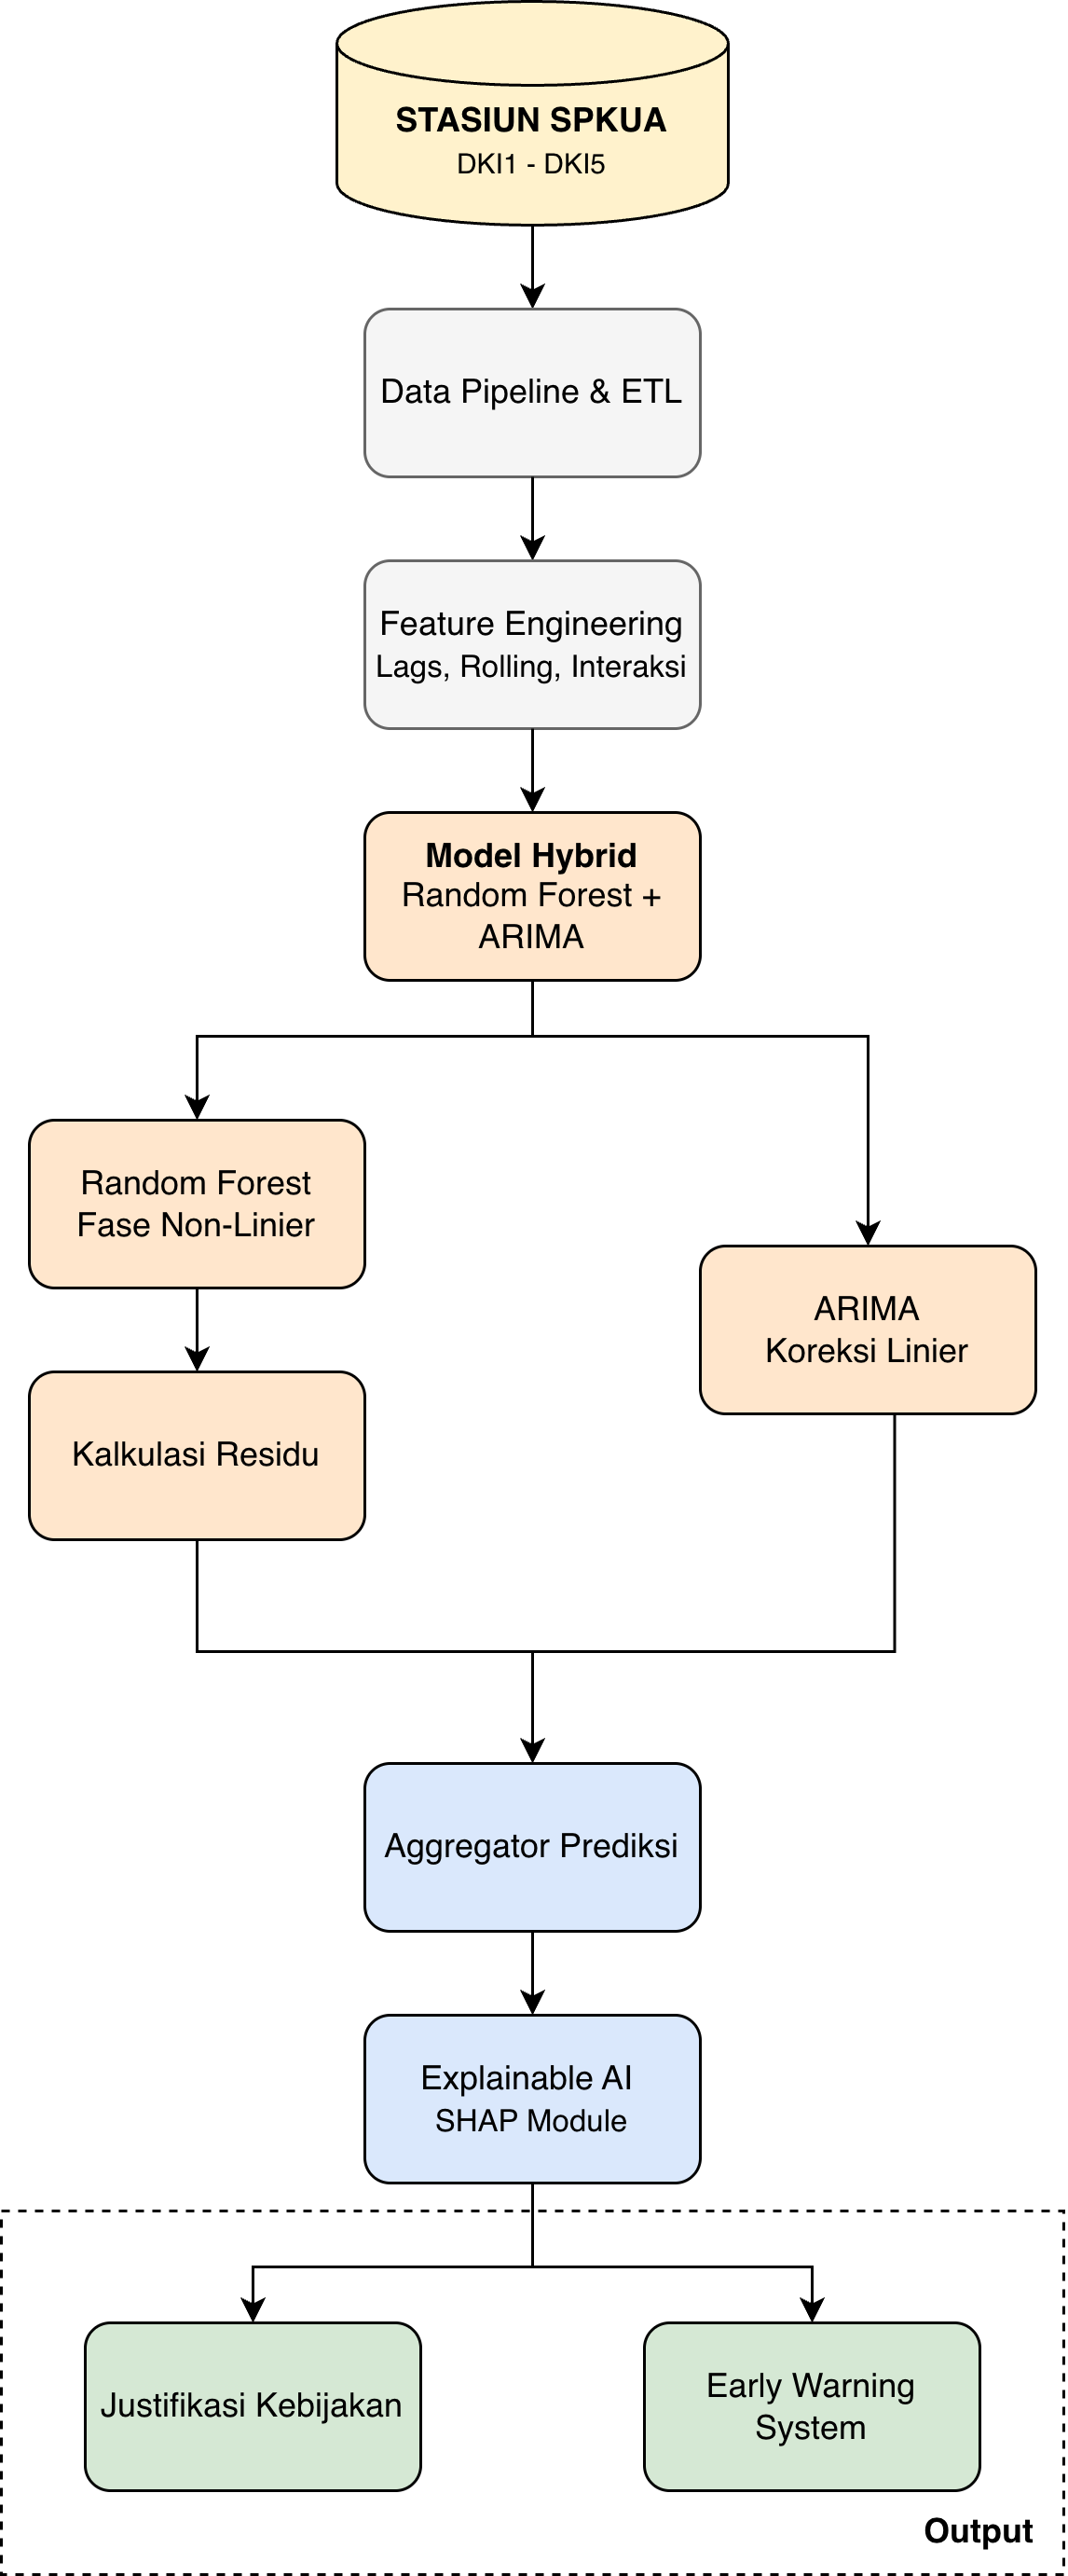
\includegraphics[width=0.4\textwidth]{images/sistem_usulan.png}
  \caption{Diagram Arsitektur Sistem Prediksi Hibrida Terintegrasi (Sistem Usulan)}
  \label{gambar:sistem_usulan}
\end{figure}

\subsection{Perbandingan Sistem}

Transformasi fungsional dari sisi peran, logika pemrosesan, dan nilai keluaran antara sistem berjalan dan sistem usulan dirangkum secara teknis pada Tabel \ref{tbl:perbandingan_arsitektur}. Tabel ini menunjukkan pergeseran karakteristik sistem dari pendekatan reaktif yang bergantung pada data mentah menuju pendekatan proaktif berbasis data multidimensi. Perbandingan ini menjadi landasan untuk menjustifikasi penggunaan model hibrida dalam pemantauan lingkungan.

\begin{table}[htbp]
\centering
\captionsetup{justification=centering}
\setlength{\tabcolsep}{6pt} 
\caption{Matriks Perbandingan Teknis Sistem Berjalan dan Sistem Usulan}
\label{tbl:perbandingan_arsitektur}

\begin{tabularx}{\textwidth}{|>{\raggedright\arraybackslash}p{2.8cm}|
                              >{\raggedright\arraybackslash}X|
                              >{\raggedright\arraybackslash}X|}
\hline
\textbf{Aspek Perancangan} & \textbf{Sistem Berjalan (\textit{Existing})} & \textbf{Sistem Usulan (\textit{Proposed})} \\
\hline
Paradigma Operasional & Reaktif; menyajikan informasi kualitas udara pasca-kejadian (\textit{post-factum}). & Proaktif; menyediakan estimasi proyeksi konsentrasi polutan harian ($t+1$). \\
\hline
Dimensi Data & Univariat tunggal berbasis parameter polutan mentah (1D). & Multivariat (15 fitur) mengintegrasikan aspek temporal dan interaksi kimiawi. \\
\hline
Mesin Pemrosesan & Kalkulasi statistik deskriptif harian untuk konversi nilai ISPU. & Hibridisasi sekuensial menggabungkan komponen linier dan non-linier. \\
\hline
Interpretabilitas & Deskriptif tanpa analisis kontribusi fitur masukan. & Transparan; analisis kontribusi fitur berbasis metode eksplorasi TreeSHAP. \\
\hline
\end{tabularx}
\end{table}

Penerapan perancangan data multidimensi menunjukkan bahwa sistem usulan menggunakan hubungan antarpolutan untuk menangkap karakteristik pola kompleks atmosfer di wilayah DKI Jakarta. Penggunaan fitur interaksi kimiawi menyediakan informasi tambahan yang tidak tersedia pada sistem berjalan yang memproses gas polutan secara terpisah. Hal ini menjadi faktor penting dalam meminimalkan kesalahan estimasi, terutama saat menghadapi variabilitas data akibat kondisi lingkungan yang berubah-ubah.

Melalui perancangan sistem yang diusulkan, luaran sistem dikembangkan dari sekadar laporan statistik menjadi instrumen prediktif untuk mendukung penentuan kebijakan. Sistem usulan menyediakan kapabilitas bagi pihak berwenang untuk merancang langkah intervensi kebijakan sebelum konsentrasi polusi mencapai ambang batas yang dapat memengaruhi kesehatan masyarakat. Integrasi fitur dan model hibrida ini menjadi alternatif pendekatan dalam pemanfaatan teknologi informasi untuk pengawasan kualitas udara perkotaan.

\section{Desain Data Pipeline dan Pemodelan UML}

Perancangan sistem dipetakan menggunakan pemodelan standar untuk mendeskripsikan aliran informasi dan interaksi fungsional sebagai solusi yang menghubungkan karakteristik rekayasa perangkat lunak dan sains data. Pendekatan ini dilakukan untuk memastikan bahwa setiap komponen sistem, mulai dari tahapan pemrosesan data hingga penyajian hasil estimasi, terdokumentasi secara teknis. Pemodelan ini juga berfungsi sebagai jembatan komunikasi antara kebutuhan fungsional sistem dengan implementasi fungsi pada tahap pengembangan.

\subsection{Diagram Alir Data (DFD)}

Aliran transformasi data dari tahapan masukan hingga keluaran dimodelkan menggunakan \textit{Data Flow Diagram} (DFD) untuk memberikan gambaran mengenai pergerakan data dalam sistem. Pemodelan ini digunakan untuk mengidentifikasi komponen masukan data, proses transformasi yang terjadi, serta keluaran yang dihasilkan untuk setiap entitas terkait. Melalui penerapan DFD, batasan operasional sistem dalam mengolah informasi polutan menjadi lebih terstruktur.

DFD Level 0 atau Diagram Konteks merepresentasikan batasan sistem secara makro dan hubungan antara sistem dengan entitas eksternal. Diagram ini menunjukkan posisi sistem sebagai unit pemrosesan data yang menerima input dari penyedia data dan mendistribusikan hasil estimasi kepada pengguna akhir. Representasi ini diperlukan untuk memahami cakupan fungsional sistem sebelum masuk ke detail teknis.

Dalam konteks sistem ini, entitas "Dinas Lingkungan Hidup / Sensor SPKUA" bertindak sebagai penyuplai data parameter polutan harian. Sistem Prediksi PM\textsubscript{10} Terintegrasi menerima data tersebut, mengeksekusi komputasi prediktif serta analitik atribusi nilai SHAP, kemudian menghasilkan keluaran berupa laporan prediksi harian dan visualisasi kontribusi fitur. Hasil akhir ini didistribusikan kepada entitas "Pemangku Kebijakan / Masyarakat" sebagai instrumen pendukung keputusan, sebagaimana ditunjukkan pada Gambar \ref{gambar:dfd_level0}.

\begin{figure}[htbp]
  \centering
  \captionsetup{justification=centering}
  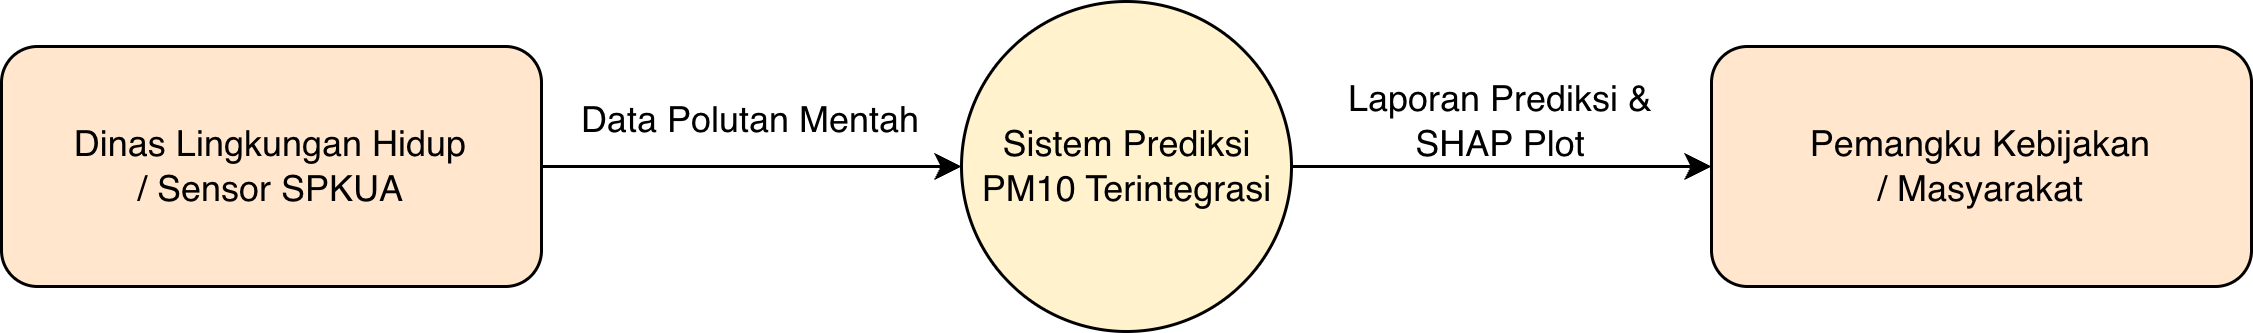
\includegraphics[width=0.8\textwidth]{images/dfd_level0.png}
  \caption{DFD Level 0 (Diagram Konteks) Sistem Prediksi PM\textsubscript{10}}
  \label{gambar:dfd_level0}
\end{figure}

\subsection{Desain Proses ETL (\textit{Extract, Transform, Load})}

Desain ETL mengatur mekanisme penyiapan data yang berasal dari kelima stasiun pemantauan (DKI1 hingga DKI5) agar dapat digunakan dalam pemodelan secara terpisah. Proses ini diperlukan mengingat data mentah dapat memiliki celah informasi akibat kendala teknis pada sensor di lapangan. Melalui tahapan ekstraksi dan transformasi, kelengkapan data dipertahankan sebelum masuk ke fase pemodelan komputasi.

Dalam rangka menangani data yang hilang tanpa menyebabkan kebocoran informasi masa depan (\textit{look-ahead bias}), dirancang sebuah algoritma imputasi dengan pendekatan \textit{historical rolling mean}. Penggunaan jendela waktu $k=5$ harian memungkinkan sistem untuk mengestimasi nilai yang hilang pada waktu $t$ murni berdasarkan tren lokal terdekat secara historis ($t-1$ hingga $t-k$) pada stasiun yang bersangkutan. Pendekatan ini digunakan untuk menjaga integritas urutan waktu kronologis dan memastikan bahwa informasi dari masa depan tidak memengaruhi proses prapemrosesan data latih.

Tahap akhir dari proses ETL adalah melakukan pembersihan dan transformasi data untuk membentuk matriks fitur prediktor yang siap digunakan. Proses prapemrosesan dilakukan secara berurutan pada setiap stasiun pemantauan guna menjaga karakteristik spasial yang unik di setiap wilayah administratif DKI Jakarta. Logika prapemrosesan dan alur imputasi data tersebut dijabarkan secara rinci pada Algoritma \ref{alg:etl-imputation}.

\begin{algorithm}[htbp]
\caption{Algoritma Prapemrosesan dan Imputasi \textit{Rolling Mean} per Stasiun}
\label{alg:etl-imputation}
\begin{algorithmic}[1] 
\Require Matriks data mentah stasiun $S = \{DKI1, DKI2, DKI3, DKI4, DKI5\}$, jendela waktu $k = 5$
\Ensure Matriks data stasiun $S$ tanpa nilai kosong (\textit{null})

\For{\textbf{each} $s \in S$}
    \For{\textbf{each} observasi waktu $t$ dari $1$ \textbf{to} $N$}
        \If{$s[t]$ is \textit{null}}
            \State $sum \gets 0$
            \For{$i = 1$ \textbf{to} $k$}
                \State $sum \gets sum + s[t-i]$
            \EndFor
            \State $s[t] \gets sum / k$ 
        \EndIf
    \EndFor
\EndFor

\State \Return $S$
\end{algorithmic}
\end{algorithm}

\subsection{Prosedur Pencegahan Kebocoran Data (\textit{Data Leakage Prevention})}
Dalam arsitektur data runtun waktu, pencegahan \textit{data leakage} (khususnya \textit{look-ahead bias}) merupakan salah satu parameter penting untuk menjaga integritas eksperimen. Sistem ini mengimplementasikan tiga tahapan pengendalian agar informasi masa depan tidak bocor ke masa lalu selama proses ETL dan pemodelan:

\begin{enumerate}
    \item {Imputasi Kausal/Historis:} Proses penanganan nilai kosong (\textit{null}) menggunakan fungsi \textit{rolling mean} berbasis data masa lalu (\textit{historical rolling mean}). Formula imputasi pada waktu $t$ murni mengevaluasi data historis dari rentang jendela $t-1$ s.d. $t-k$. Nilai masa depan pada $t+1$ s.d. $t+k$ sama sekali tidak diikutsertakan dalam pembobotan interpolasi sensor.
    \item {Feature Engineering Bebas Bias Temporal:} Seluruh kalkulasi variabel turunan statistik bergerak (\textit{Rolling Mean} 3-hari dan 7-hari) dikonfigurasi menggunakan parameter fungsi Python \textit{closed='left'}. Aturan ini memastikan titik perhitungan pada hari ini ($t$) murni mengagregasi data historis hari-hari ke belakang tanpa menyertakan nilai target hari ini yang akan diprediksi.
    \item {Isolasi Standardisasi Skala (\textit{Scaling Isolation}):} Guna mencegah kebocoran informasi distribusi statistik dari set validasi atau pengujian ke dalam set pelatihan, instrumen penyelarasan nilai (\textit{StandardScaler}) dilatih secara ketat hanya menggunakan subset data pelatihan (\textit{scaler.fit\_transform(X\_train)}). Data evaluasi lainnya kemudian ditransformasikan secara pasif menggunakan parameter rata-rata dan deviasi standar yang diekstrak dari fase pelatihan (\textit{scaler.transform(X\_val)}), tanpa melakukan kalkulasi ulang distribusi pada data di luar set latih.
\end{enumerate}

\subsection{Activity Diagram Pemodelan Hibrida}

Logika fase komputasi model pada saat mode pelatihan (\textit{training}) didokumentasikan melalui \textit{Activity Diagram} untuk menggambarkan urutan aktivitas secara sekuensial. Diagram ini memberikan gambaran mengenai alur kerja sistem dalam mempelajari karakteristik data dari tahap awal hingga model siap digunakan untuk melakukan estimasi. Pemisahan aktivitas dilakukan dengan tujuan menghindari tumpang tindih fungsi dalam arsitektur hibrida sekuensial yang dikembangkan. Rincian alur kerja serta tahapan sekuensial pada proses pelatihan model ini disajikan secara visual pada Gambar \ref{gambar:activity_diagram}.

Berdasarkan alur yang dirancang pada Gambar \ref{gambar:activity_diagram}, proses komputasi berjalan secara berurutan untuk menjaga keteraturan fungsi tiap modul. Setelah tahapan rekayasa fitur (\textit{feature engineering}) selesai dieksekusi, data dikirim ke modul \textit{Random Forest} Regresi untuk fase pelatihan primer guna menghasilkan estimasi nilai awal, yang kemudian dilanjutkan dengan kalkulasi sisaan (\textit{residual}) melalui selisih antara nilai aktual dan hasil prediksi tersebut. Deret sisaan galat ini selanjutnya diproses menggunakan model statistik ARIMA pada fase sekunder untuk menangkap komponen linier temporal yang belum terurai oleh percabangan pohon keputusan. Penggabungan dua metode dengan karakteristik berbeda ini diterapkan agar diperoleh hasil estimasi akhir dengan akumulasi galat yang terkendali, di mana keseluruhan alur pelatihan diakhiri dengan penyimpanan konfigurasi parameter dari kedua model (\textit{Saved Model}) untuk fase inferensi harian secara berkala.

\begin{figure}[htbp]
  \centering
  \captionsetup{justification=centering}
  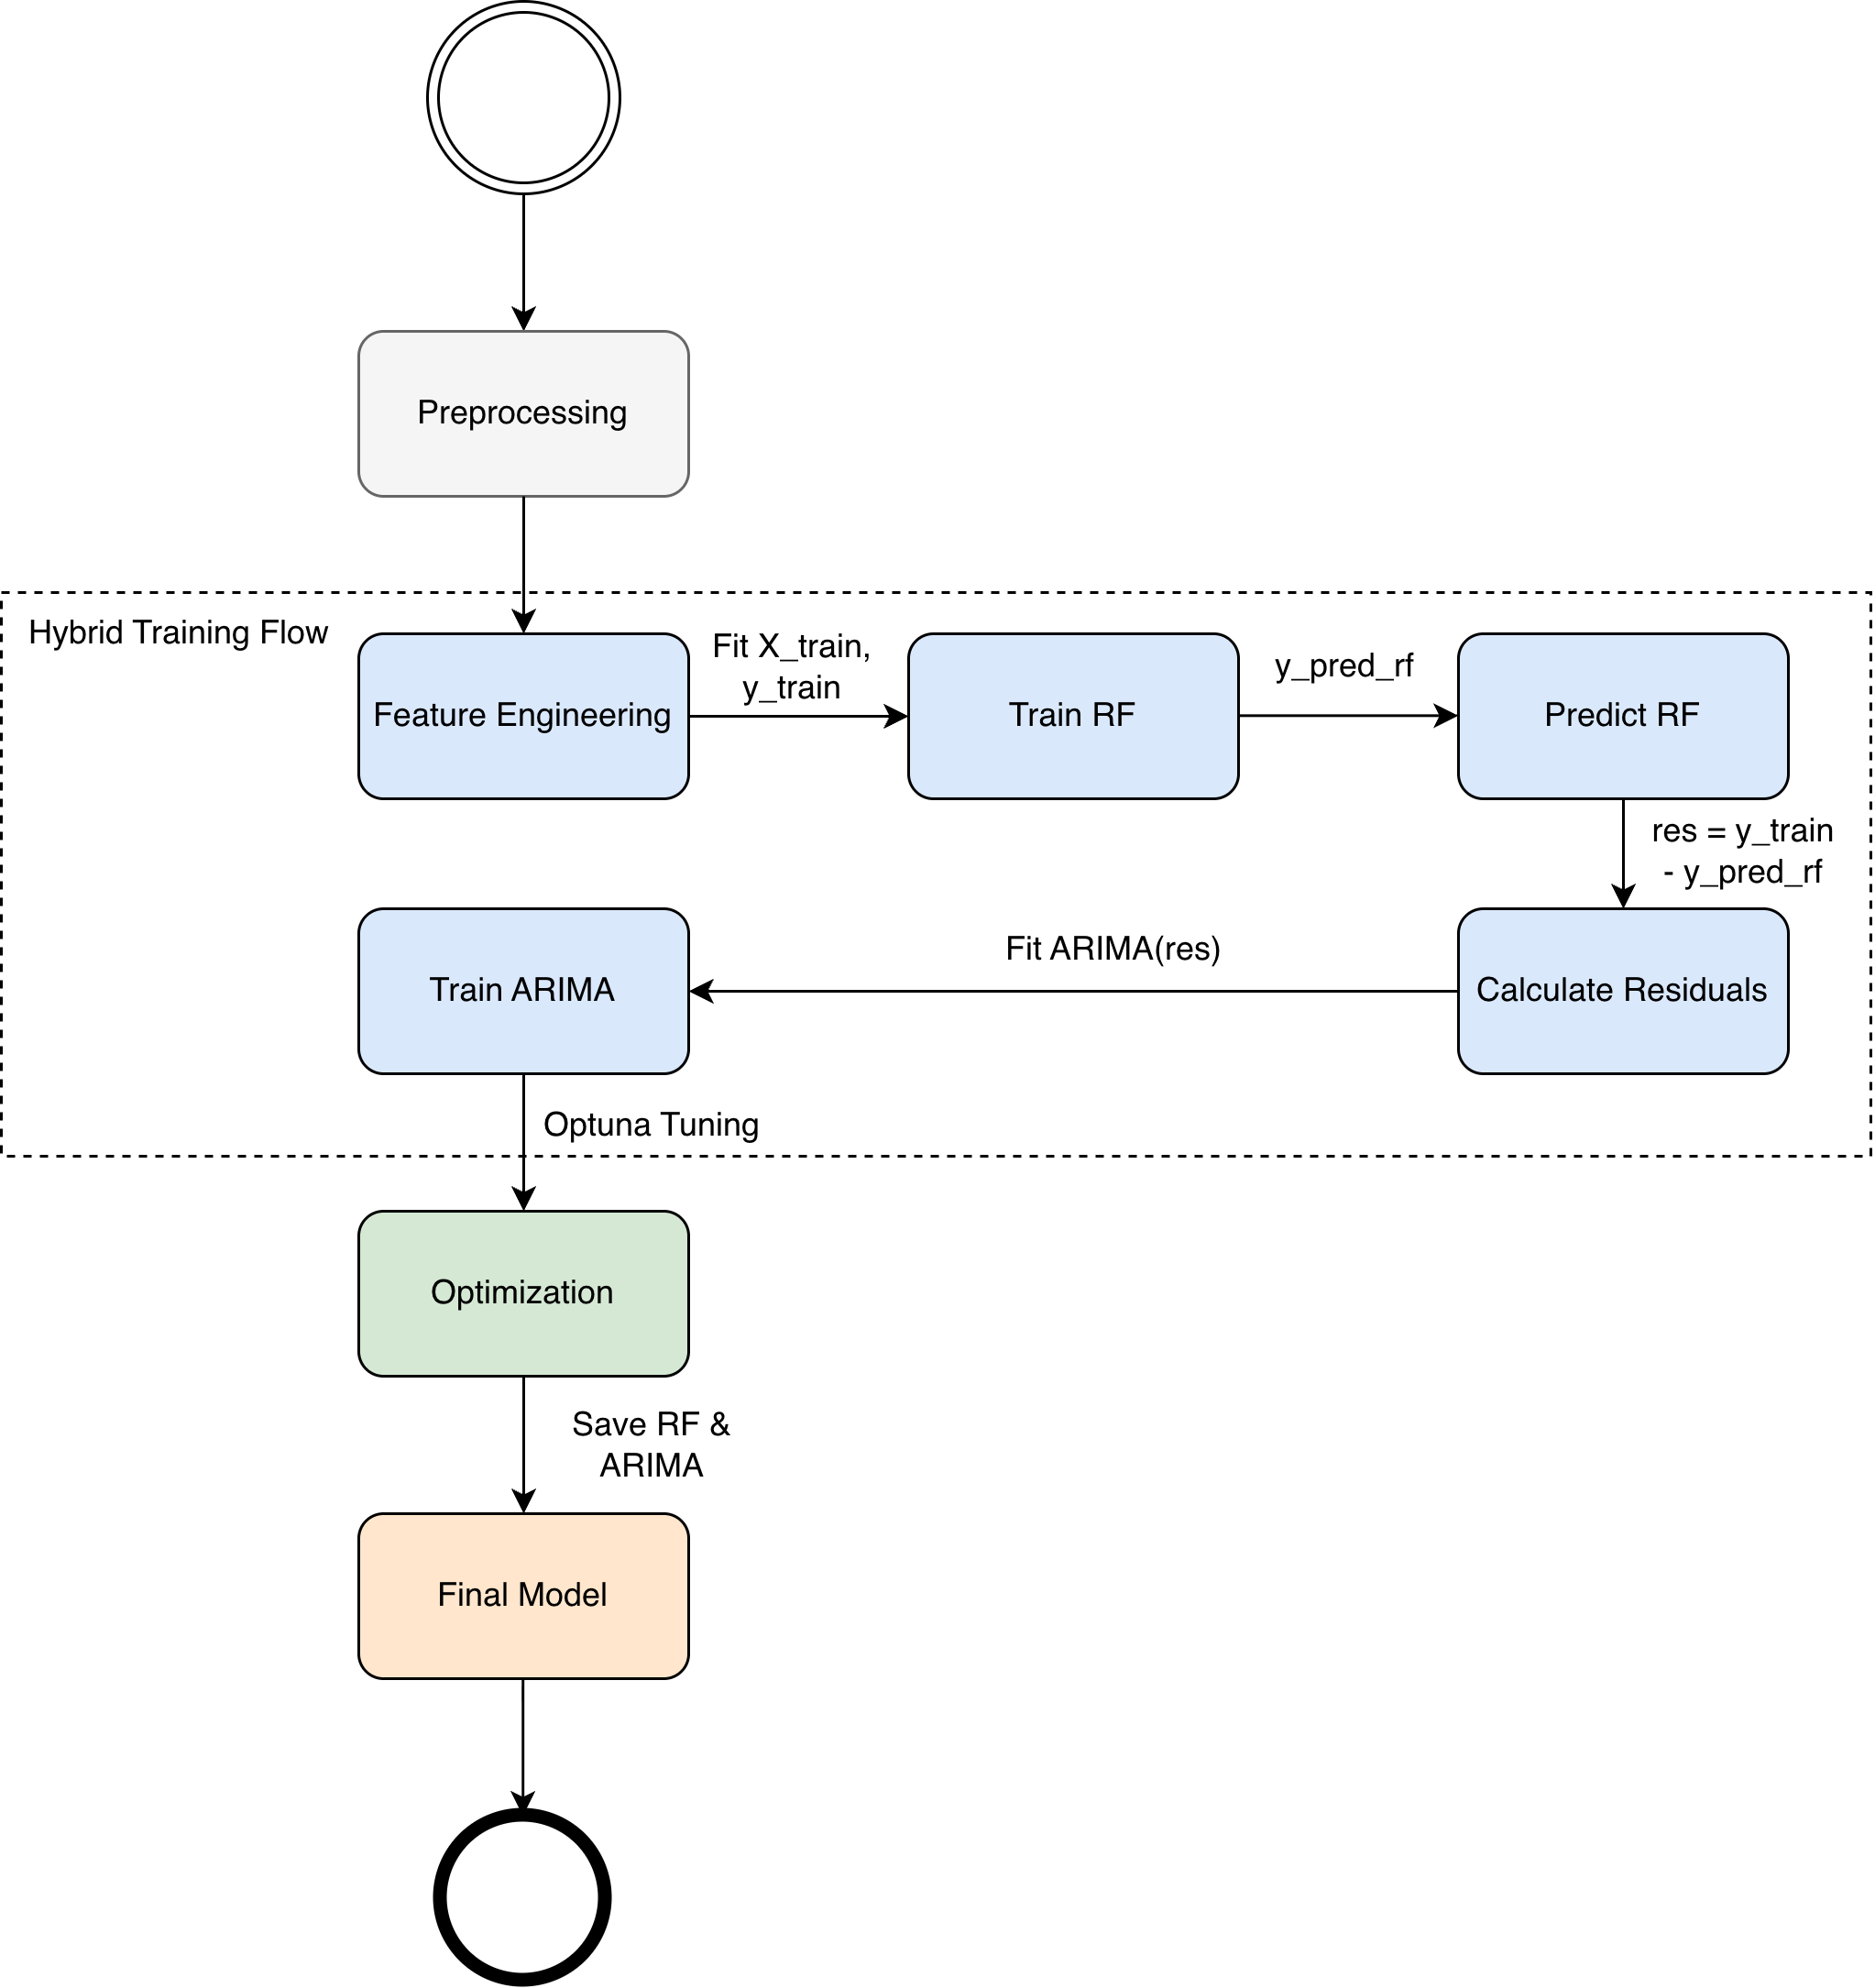
\includegraphics[width=0.6\textwidth]{images/activity_diagram.png}
  \caption{\textit{Activity Diagram} Alur Pelatihan Model Hibrida Sekuensial}
  \label{gambar:activity_diagram}
\end{figure}

\subsection{Sequence Diagram Sistem Inferensi Berkala}

Prosedur operasional sistem pada saat melakukan peramalan harian divisualisasikan melalui \textit{Sequence Diagram} untuk menunjukkan interaksi antar-modul. Diagram ini menggambarkan alur penyampaian pesan dan koordinasi berbagai komponen perangkat lunak dalam merespons permintaan estimasi konsentrasi polutan. Melalui pemodelan urutan ini, hubungan kronologis antar-komponen serta eksistensi elemen perangkat lunak selama proses inferensi berlangsung dapat ditelaah secara terstruktur, sebagaimana ditampilkan secara mendetail pada Gambar \ref{gambar:sequence_diagram}.

\begin{figure}[htbp]
  \centering
  \captionsetup{justification=centering}
  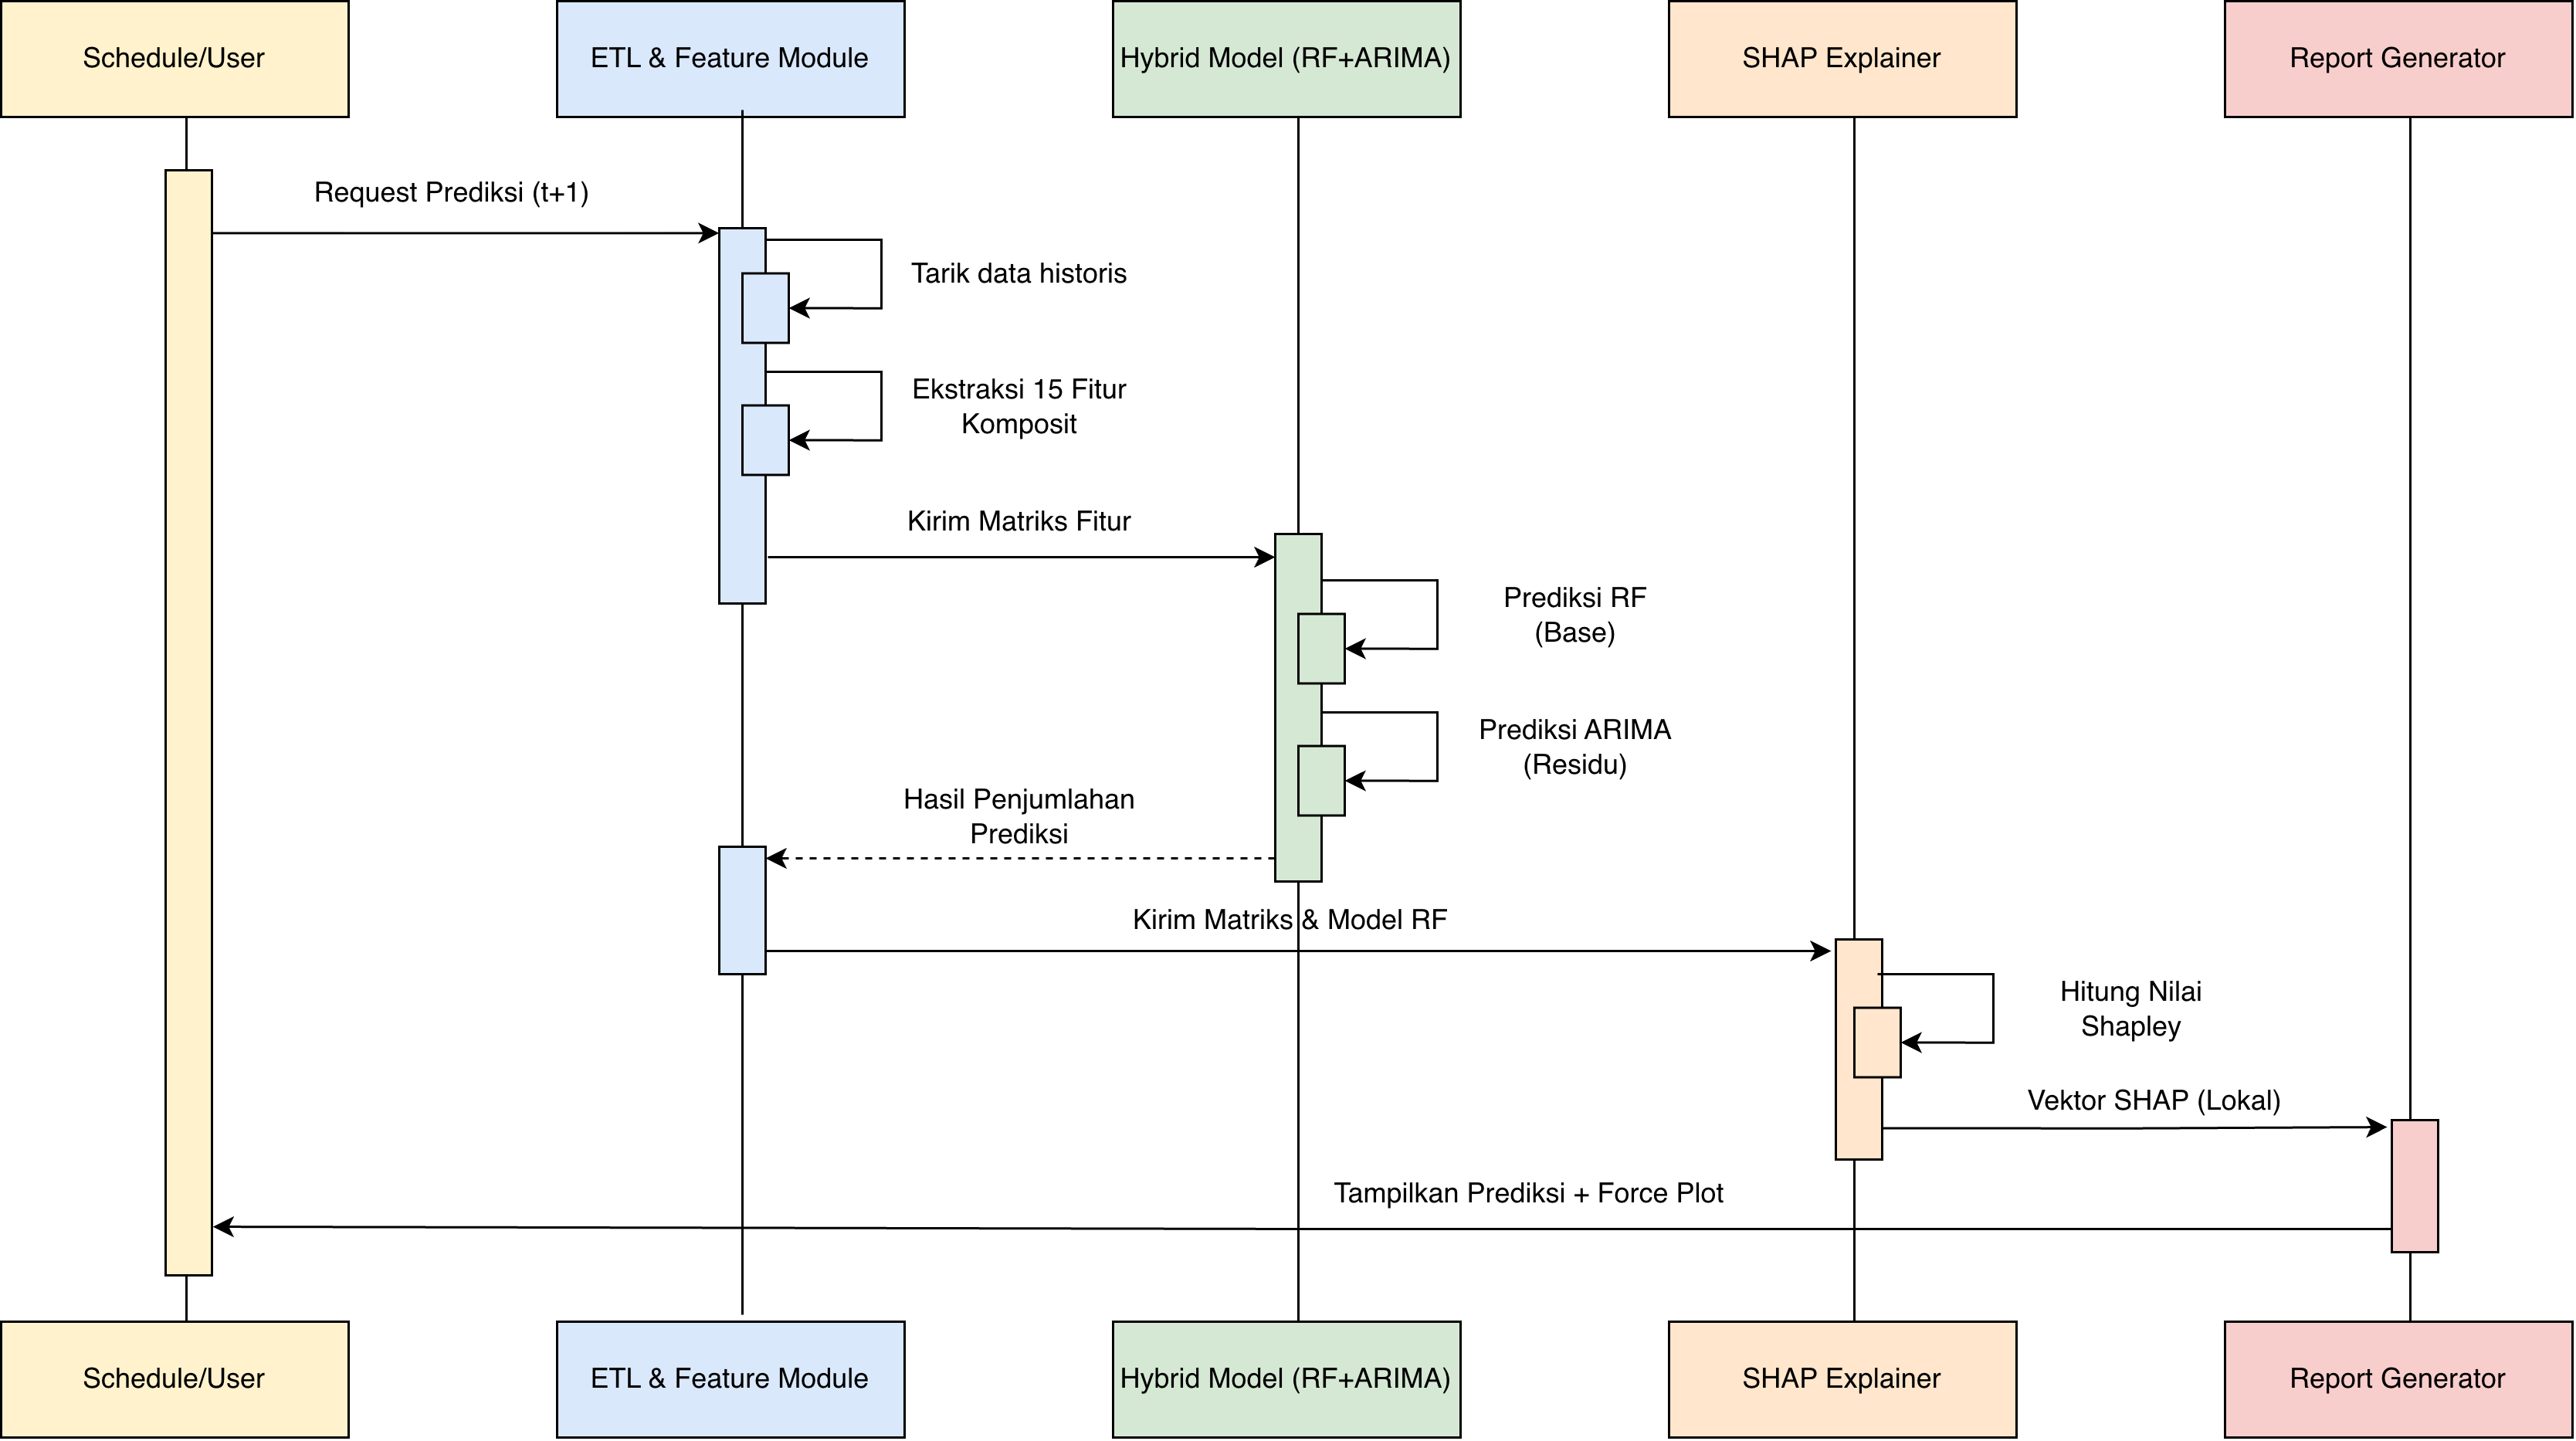
\includegraphics[width=0.7\textwidth]{images/sequence_diagram.png}
  \caption{\textit{Sequence Diagram} Proses Inferensi Prediksi Harian}
  \label{gambar:sequence_diagram}
\end{figure}

\newpage

Berdasarkan tahapan urutan yang digambarkan pada Gambar \ref{gambar:sequence_diagram}, alur inferensi berkala (\textit{automated batch processing}) diawali ketika komponen penjadwal (\textit{Scheduler}) memicu modul ETL untuk menarik tujuh hari riwayat data terakhir dari basis data stasiun. Modul prediksi kemudian memuat konfigurasi parameter model \textit{Random Forest} Regresi dan ARIMA dari memori penyimpanan untuk menjalankan proses kalkulasi secara sekuensial, di mana hasil dari kedua model tersebut dijumlahkan untuk menghasilkan nilai prediksi tunggal yang merepresentasikan konsentrasi PM\textsubscript{10} untuk horizon satu hari ke depan ($t+1$). Tahap akhir dari rangkaian proses ini melibatkan modul penjelasan model untuk mengkalkulasi pengaruh setiap fitur masukan terhadap hasil estimasi yang dikeluarkan, sebelum seluruh informasi dikemas menjadi sebuah laporan terpadu yang memuat nilai prediksi beserta visualisasi kontribusi fiturnya.

\section{Spesifikasi Algoritmik Rekayasa Fitur}

Bagian ini merumuskan transformasi variabel mentah menjadi matriks fitur yang memiliki varians informasi temporal dan karakteristik kimiawi untuk memproses sifat data deret waktu PM\textsubscript{10}. Rekayasa fitur dilakukan untuk menyediakan variabel prediktor tambahan yang tidak termuat secara langsung pada data mentah, namun memiliki pengaruh terhadap fluktuasi nilai kualitas udara di Jakarta. Dengan memperluas dimensi masukan melalui fitur turunan, model hibrida diharapkan mampu menghasilkan estimasi yang stabil.

\subsection{Matriks Transformasi Fitur}

Transformasi variabel mentah menjadi matriks fitur dilakukan untuk mengelola karakteristik data kualitas udara PM\textsubscript{10} yang memiliki varians fluktuasi dan dependensi musiman. Rekayasa fitur dalam penelitian ini bertujuan untuk mengekstraksi informasi temporal dan kimiawi berkala yang tidak terlihat secara langsung pada observasi harian harian, namun berpengaruh terhadap persistensi polutan di atmosfer. Melalui perluasan dimensi input, model hibrida dapat menangkap dependensi temporal dan korelasi antarpolutan secara lebih komprehensif.

Rancangan fitur secara teoretis dibagi ke dalam empat kategori utama untuk memberikan konteks prediktif. Kategori tersebut meliputi fitur \textit{lag} untuk menangkap pengaruh variabel hari sebelumnya, statistik \textit{rolling window} untuk memetakan tren mingguan, interaksi kimiawi untuk merepresentasikan hubungan antar gas polutan, serta penanda temporal untuk mengidentifikasi aktivitas masyarakat urban. Pembagian kategori ini dilakukan agar setiap variabel yang dihasilkan memiliki landasan teoretis yang sesuai dengan kondisi lingkungan perkotaan.

Matriks desain fitur yang dikembangkan mengintegrasikan total 15 fitur komposit yang disusun berdasarkan karakteristik data ISPU di DKI Jakarta. Tabel \ref{tbl:matriks_fitur} merangkum spesifikasi teknis dari variabel-variabel turunan tersebut beserta fungsinya dalam model. Penentuan variabel ini menjadi tahapan dalam memitigasi galat prediksi yang muncul akibat perubahan pola emisi kendaraan dan industri yang dinamis, sebagaimana dirinci pada tabel berikut.

\begin{table}[htbp]
\centering
\captionsetup{justification=centering}
\setlength{\tabcolsep}{6pt}
\caption{Matriks Desain Fitur Komposit Hibrida}
\label{tbl:matriks_fitur}

\begin{tabularx}{\textwidth}{|>{\raggedright\arraybackslash}p{2.8cm}|
                              >{\raggedright\arraybackslash}p{3.8cm}|
                              >{\raggedright\arraybackslash}X|}
\hline
\textbf{Kategori Fitur} & \textbf{Nama Variabel} & \textbf{Justifikasi Fisis / Fungsi} \\
\hline
Lag Temporal & \texttt{pm10\_lag1}, \texttt{pm10\_lag2}, \texttt{pm10\_lag7} & Menangkap efek persistensi massa polutan harian dan pengaruh siklus komuter mingguan. \\
\hline
Statistik Berjalan & \texttt{pm10\_ma3}, \texttt{pm10\_ma7}, \texttt{pm10\_std7} & Memetakan tren pergerakan nilai polusi jangka pendek, mingguan, serta tingkat volatilitas data. \\
\hline
Interaksi Kimia & \texttt{co\_times\_o3} & Representasi aktivitas fotokimia primer dan laju pembentukan partikulat sekunder di atmosfer. \\
\hline
Penanda Temporal & \texttt{month}, \texttt{season}, \texttt{is\_weekend} & Mengidentifikasi variasi musiman makro (presipitasi) dan penurunan mobilitas urban akhir pekan. \\
\hline
\end{tabularx}
\end{table}

\subsection{Logika Pembangkitan Fitur Temporal dan Interaksi}

Polusi udara di wilayah metropolitan dipengaruhi oleh emisi primer dan reaksi pembentukan partikulat sekunder yang terjadi akibat interaksi kimiawi antar gas polutan. Pembangkitan fitur komposit dalam penelitian ini dirancang sebagai upaya untuk merepresentasikan dinamika tersebut, khususnya pada interaksi antara gas Karbon Monoksida dan Ozon Permukaan yang menjadi salah satu penanda fluktuasi partikulat. Melalui pendekatan perkalian antarvariabel gas ini, model diharapkan dapat mengidentifikasi pola data yang mendekati karakteristik kondisi di lapangan tanpa harus memperdalam struktur percabangan pohon keputusan.

Selain variabel kimiawi, faktor aktivitas temporal berupa siklus mingguan dan bulanan juga dimasukkan sebagai fitur tambahan untuk mengamati indikasi variasi beban emisi dari sektor transportasi. Langkah ini dilakukan dengan tujuan agar setiap baris data memiliki penanda waktu, sehingga model dapat membedakan kecenderungan pola polusi antara hari kerja dan akhir pekan. Integrasi fitur temporal ini berfungsi sebagai informasi masukan pelengkap bagi algoritma \textit{Random Forest} Regresi. Prosedur rekayasa fitur beserta alur kerjanya secara berurutan ditunjukkan pada Algoritma \ref{alg:fitur-komposit} dan diagram alir Gambar \ref{gambar:flowchart_fe} di bawah ini.

\begin{algorithm}[htbp]
\caption{Pembangkitan Fitur Interaksi dan Temporal}
\label{alg:fitur-komposit}
\begin{algorithmic}[1] 
\Require Matriks $X$ dengan parameter dasar ($\text{PM}_{10}$, $\text{CO}$, $\text{O}_3$, $\text{SO}_2$, $\text{NO}_2$) terindeks waktu $t$
\Ensure Matriks $X_{new}$ yang telah dikombinasikan dengan fitur komposit
\For{$t = 1$ \textbf{to} $N$}
    \State $X_{new}[t].month \gets \text{EkstrakBulan}(t)$
    \State $X_{new}[t].season \gets \text{PenentuanMusim}(t)$
    \State $day \gets t \pmod 7$
    \If{$day = 5$ \textbf{or} $day = 6$}
        \State $X_{new}[t].is\_weekend \gets 1$
    \Else
        \State $X_{new}[t].is\_weekend \gets 0$
    \EndIf
    \State $X_{new}[t].co\_times\_o3 \gets X[t].CO \times X[t].O_3$
\EndFor
\State \Return $X_{new}$
\end{algorithmic}
\end{algorithm}

\begin{figure}[htbp]
  \centering
  \captionsetup{justification=centering}
  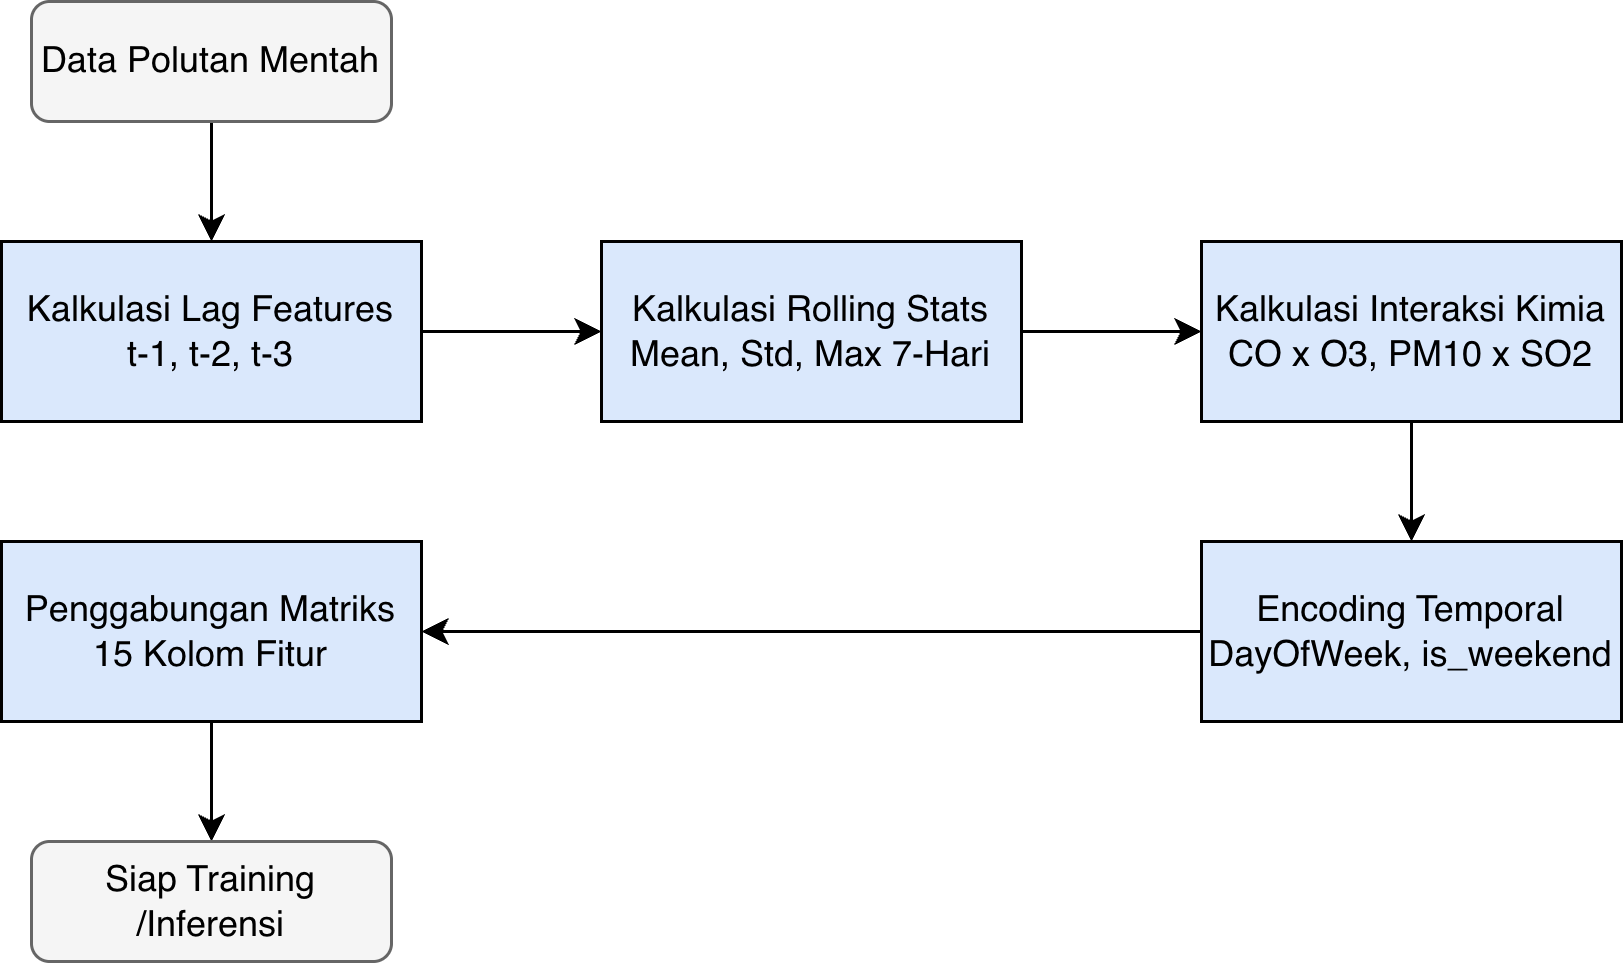
\includegraphics[width=0.6\textwidth]{images/flowchart.png}
  \caption{Alur Logika Pembangkitan Fitur Komposit}
  \label{gambar:flowchart_fe}
\end{figure}

\newpage

Diagram alir tersebut memperjelas bahwa implementasi logika pembangkitan fitur dieksekusi secara otomatis setelah tahap prapemrosesan data selesai. Urutan eksekusi dikonstruksi mulai dari pengolahan data \textit{lag}, perhitungan statistik bergerak pada jendela waktu yang ditentukan, hingga kalkulasi akhir fitur interaksi antarpolutan. Struktur prosedur ini dirancang untuk menjaga konsistensi hasil transformasi matriks fitur pada setiap iterasi eksperimen dan memastikan kerangka pemodelan tetap stabil.

\subsection{Mekanisme Standardisasi Skala}

Seluruh matriks fitur yang telah dibangkitkan memiliki rentang nilai yang bervariasi, mulai dari satuan konsentrasi indeks gas polutan hingga penanda biner untuk variabel waktu harian. Perbedaan skala antar dimensi masukan ini dapat memengaruhi stabilitas pada proses konvergensi model dan pengaruh fitur dengan nilai absolut besar terhadap hasil estimasi. Oleh karena itu, diperlukan tahapan standardisasi untuk menyelaraskan distribusi seluruh variabel masukan sebelum memasuki fase pelatihan model hibrida.

Mekanisme standardisasi yang diterapkan dalam perancangan ini adalah \textit{Z-Score Standardization} (\textit{StandardScaler}). Metode ini mengubah distribusi setiap fitur sehingga memiliki nilai rata-rata nol dan deviasi standar satu, tanpa menghilangkan karakteristik distribusi aslinya. Proses penskalaan ini dilakukan secara terpisah antara data latih dan data uji untuk meminimalkan risiko terjadinya kebocoran informasi masa depan (\textit{look-ahead bias}) yang dapat menyebabkan hasil evaluasi menjadi bias.

Penggunaan standardisasi skala digunakan untuk mendukung stabilitas numerik pada algoritma regresi dan membantu proses pencarian hiperparameter yang sesuai melalui Optuna. Dengan menyamakan rentang nilai, kontribusi setiap fitur terhadap target prediksi $PM_{10}$ dapat dievaluasi secara proporsional oleh model \textit{Random Forest} Regresi maupun ARIMA. Konstruksi matematis dari transformasi standardisasi skala ini mengikuti prinsip statistika sebagaimana diturunkan pada Persamaan \ref{eq:standardization}.

\begin{equation}
z = \frac{x - \mu}{\sigma}
\label{eq:standardization}
\end{equation}
\eqcaption{Formulasi Standardisasi Skala Menggunakan Z-Score}

\section{Desain Arsitektur Hibrida Sekuensial}

Pemodelan dirancang menggunakan pendekatan sekuensial di mana algoritma ansambel berbasis pohon dan fungsi diferensi stokastik linier bekerja secara komplementer untuk memetakan pola polusi udara. Arsitektur hibrida ini dikonstruksi untuk memisahkan komponen data non-linier dari komponen linier yang bersifat temporal pada deret waktu PM\textsubscript{10}. Melalui penggabungan dua pendekatan pemodelan yang berbeda, sistem diarahkan untuk mampu menghasilkan estimasi dengan nilai kesalahan yang rendah dibandingkan penggunaan model tunggal murni.

Integrasi sekuensial ini dimulai dengan pemodelan fase primer yang bertujuan untuk memetakan komponen varians utama dari data. Hasil keluaran dari fase primer tersebut kemudian diproses lebih lanjut untuk mengidentifikasi nilai residu yang masih menyimpan karakteristik informasi tertentu. Tahapan ini dilakukan agar setiap algoritma bekerja pada domain data yang sesuai dengan karakteristik matematis masing-masing, guna meminimalkan risiko ketidaksesuaian pola data.

Aliran kerja arsitektur hibrida ini secara sistematis mencakup fase pelatihan primer, perhitungan residu, pelatihan fase sekunder, hingga integrasi akhir hasil prediksi. Penggunaan metode sekuensial ini juga memfasilitasi proses pencarian parameter yang terstruktur bagi kedua model. Struktur desain ini menjadi fondasi utama dalam mencapai target penaksiran nilai galat peramalan kualitas udara di wilayah DKI Jakarta.

\subsection{Desain Fase Primer (\textit{Random Forest}) Regresi}

Pada fase pertama, keseluruhan matriks fitur $X_{train}$ hasil rekayasa dimasukkan ke model \textit{Random Forest Regressor} (Regresi) untuk memetakan hubungan fungsional terhadap target PM\textsubscript{10}. Algoritma ini dipilih sebagai pembelajar primer karena karakteristiknya dalam memproses data multidimensi dan kemampuannya dalam mengidentifikasi tingkat kepentingan fitur secara otomatis. Proses ini fokus pada penangkapan fluktuasi polusi yang dipengaruhi oleh interaksi kimiawi dan variabel temporal.

Konstruksi model fase primer melibatkan pembentukan sejumlah pohon keputusan yang bekerja secara independen melalui skema \textit{bagging}. Setiap pohon memberikan estimasi nilai polutan, yang kemudian dirata-ratakan untuk menghasilkan satu nilai estimasi nilai awal (\textit{base prediction}). Pendekatan ansambel ini digunakan untuk mereduksi varians dan menjaga stabilitas prediksi pada data polusi udara yang memiliki fluktuasi harian.

Ruang inisialisasi parameter pada fase ini dirancang untuk memfasilitasi proses pencarian di tahap berikutnya. Parameter utama yang dikonfigurasi meliputi jumlah estimator (\texttt{n\_estimators}) untuk menentukan banyaknya pohon, serta kedalaman maksimum pohon (\texttt{max\_depth}) untuk mengontrol kompleksitas model. Pengaturan parameter pada fase primer ini penting karena akan menentukan karakteristik residu yang akan diolah oleh model fase sekunder.

\subsection{Logika Kalkulasi Residu Temporal}

Integrasi sekuensial antara komponen non-linier dan linier dalam pemodelan hibrida didasarkan pada prinsip jumlahan komponen varians data target PM\textsubscript{10}. Berdasarkan metode dekomposisi asimilasi, deret waktu aktual dipandang sebagai gabungan dari pola non-linier dan dependensi linier temporal. Dengan menjumlahkan hasil estimasi fase primer dan koreksi fase sekunder, model hibrida menyusun akumulasi proyeksi akhir. Formulasi jumlahan aditif beserta penjabaran komponen perhitungan matematis model hibrida secara eksplisit didefinisikan pada Persamaan \ref{eq:hybrid_sum}.

\begin{equation}
\begin{aligned}
\hat{Y}_{hybrid, t} &= \hat{N}_t + \hat{L}_t \\[2ex]
\text{dengan:} \quad \hat{N}_t &= \frac{1}{B} \sum_{b=1}^{B} T_b(X_t) \\[2ex]
\hat{L}_t &= c + \sum_{i=1}^{p} \phi_i \Delta^d e_{t-i} + \sum_{j=1}^{q} \theta_j \epsilon_{t-j} \\[3ex]
\text{Sehingga substitusi akhir } &\text{secara utuh didefinisikan sebagai:} \\[2ex]
\hat{Y}_{hybrid, t} = \left[ \frac{1}{B} \sum_{b=1}^{B} T_b(X_t) \right] &+ \left[ c + \sum_{i=1}^{p} \phi_i \Delta^d e_{t-i} + \sum_{j=1}^{q} \theta_j \epsilon_{t-j} \right]
\end{aligned}
\label{eq:hybrid_sum}
\end{equation}
\eqcaption{Formulasi Prediksi Akhir dan Eksplorasi Matematis Arsitektur Hibrida Sekuensial}

Pada formulasi di atas, $B$ merepresentasikan jumlah estimator pohon (\textit{n\_estimators}), $T_b(X_t)$ merupakan luaran prediksi dari pohon ke-$b$ dengan masukan matriks fitur multidimensi $X_t$, $c$ adalah nilai konstanta, $\phi_i$ dan $\theta_j$ melambangkan koefisien parameter \textit{Autoregressive} (AR) dan \textit{Moving Average} (MA), $\Delta^d e_{t-i}$ merupakan nilai residu terdiferensiasi sebanyak $d$ kali, serta $\epsilon_{t-j}$ melambangkan komponen \textit{white noise}.

Data residu ($e_t = Y_t - \hat{N}_t$) dalam konteks kualitas udara Jakarta mencerminkan komponen linier temporal sisa yang tidak terurai oleh percabangan pohon keputusan pada fase primer. Fenomena fisik atmosfer, seperti penumpukan partikulat di dekat permukaan tanah pada lapisan batas planet yang stabil, kerap menyisakan pola autokorelasi linier yang terlewat dari pemodelan berbasis pohon yang terfokus pada fluktuasi nilai harian. Melalui pemrosesan deret sisaan galat ini menggunakan komponen ARIMA pada fase sekunder, sistem melakukan penyesuaian nilai guna meminimalkan sisa kesalahan estimasi akhir secara keseluruhan. Logika komputasi kalkulasi residu dan penggabungan proyeksi sekuensial tersebut dijabarkan secara rinci pada Algoritma \ref{alg:kalkulasi-residu}.

\begin{algorithm}[htbp]
\caption{Kalkulasi Residu Hibrida Sekuensial}
\label{alg:kalkulasi-residu}
\begin{algorithmic}[1]
\Require Target aktual $Y$, Matriks fitur $X$, Model tersimpan $RF$ dan $ARIMA$
\Ensure Hasil prediksi hibrida akhir $Y_{hybrid}$

\State $\hat{N} \gets RF.predict(X)$ 
\State $res \gets$ array kosong berukuran $|Y|$
\For{$t = 1$ \textbf{to} $|Y|$}
    \State $res[t] \gets Y[t] - \hat{N}[t]$ 
\EndFor

\State $\hat{L} \gets ARIMA.predict(res)$ 

\State $Y_{hybrid} \gets$ array kosong
\For{$t = 1$ \textbf{to} $|Y|$}
    \State $Y_{hybrid}[t] \gets \hat{N}[t] + \hat{L}[t]$
\EndFor

\State \Return $Y_{hybrid}$
\end{algorithmic}
\end{algorithm}

\subsection{Desain Fase Sekunder (ARIMA)}

Deret residu hasil komputasi yang telah dipisahkan dari pola data kemudian diuji stasioneritasnya sebagai syarat dalam pemodelan statistik. Pengujian dilakukan menggunakan metode \textit{Augmented Dickey-Fuller} (ADF) untuk menentukan apakah deret sisaan tersebut memerlukan proses pembedaan (\textit{differencing}). Hasil uji ADF menentukan nilai parameter $d$ yang diperlukan agar data residu memenuhi asumsi stasioneritas.

Setelah kondisi stasioner terpenuhi, model ARIMA digunakan untuk mengekstraksi keterikatan temporal melalui parameter autokorelasi (\textit{Auto-Regressive}) dan rata-rata bergerak (\textit{Moving Average}). Fase ini fokus pada penangkapan dependensi temporal linear yang masih terdapat dalam data residu. Penggunaan ARIMA sebagai model sekunder bertujuan untuk melakukan penyetelan halus (\textit{fine-tuning}) terhadap estimasi awal yang dihasilkan oleh fase primer.

Konfigurasi parameter $(p, d, q$) pada fase sekunder ini diatur secara dinamis untuk menyesuaikan dengan karakteristik residu pada setiap stasiun pemantauan. Hal ini dilakukan agar model ARIMA mampu beradaptasi dengan tingkat persistensi polutan yang bervariasi di wilayah DKI Jakarta. Hasil peramalan dari fase sekunder ini kemudian dijumlahkan dengan hasil fase primer untuk menghasilkan luaran sistem akhir.

\subsection{Desain Orkestrasi Penyetelan Parameter Menggunakan Optuna}

Penyetelan parameter dilakukan untuk menghindarkan model dari keterbatasan pencarian manual atau pencarian heuristik konvensional yang memerlukan waktu lama. Dalam penelitian ini, diimplementasikan kerangka pencarian probabilitas berbasis Bayesian menggunakan pustaka Optuna untuk mencari kombinasi parameter bagi \textit{Random Forest} Regresi dan ARIMA secara bersamaan. Pendekatan ini bekerja dengan mengevaluasi performa model berdasarkan fungsi objektif khusus yang meminimalkan galat prediksi berupa metrik \textit{Root Mean Squared Error} (RMSE) pada data validasi yang diekstrak melalui skema validasi silang di dalam arsitektur hibrida sekuensial.

Proses eksplorasi tersebut mengandalkan algoritma \textit{Tree-structured Parzen Estimator} (TPE) yang secara probabilistik mengarahkan pemilihan parameter ke ruang nilai yang berpotensi menghasilkan nilai galat rendah berdasarkan riwayat percobaan sebelumnya. Melalui mekanisme ini, pencarian parameter orde $p$ dan $q$ pada komponen ARIMA serta batas struktural berupa jumlah pohon keputusan (\texttt{n\_estimators}) dan kedalaman maksimum (\texttt{max\_depth}) pada komponen \textit{Random Forest} dapat dilakukan secara otomatis. Tahap penyesuaian parameter berbasis probabilitas ini ditujukan untuk membantu stabilitas konvergensi model serta mempercepat waktu komputasi dibandingkan dengan metode pencarian konvensional, sehingga menghasilkan konfigurasi model yang memiliki kemampuan generalisasi saat dihadapkan pada data baru.

\subsection{Justifikasi Efisiensi Optuna pada Ruang Hiperparameter Kombinasi}

Dalam arsitektur hibrida sekuensial ini, terdapat kombinasi parameter struktural dari dua ranah algoritma yang berbeda secara simultan: parameter struktur pohon \textit{Random Forest} Regresi (\texttt{n\_estimators} dan \texttt{max\_depth}) serta parameter orde polinomial statistik \textit{ARIMA} ($p$ dan $q$). Jika dievaluasi menggunakan \textit{Grid Search}, ruang pencarian kombinasi dimensi silang ini akan berlipat ganda secara eksponensial ($O(A \times B)$), yang memicu tingginya konsumsi memori dan waktu komputasi yang kurang efisien untuk pemrosesan operasional harian.

Pustaka Optuna digunakan sebagai pendekatan untuk menangani kendala kompleksitas tersebut dengan menerapkan pencarian berbasis optimasi Bayesian Parzen Estimator (TPE). TPE secara dinamis membangun fungsi probabilitas penggerak yang mempelajari riwayat hasil kombinasi hiperparameter dari percobaan-percobaan sebelumnya. Optuna memfokuskan pencarian berikutnya secara terarah pada ruang parameter yang memiliki probabilitas tinggi untuk meminimalkan fungsi kesalahan galat (\textit{objective function} berupa RMSE harian), serta memangkas percobaan yang tidak menunjukkan perbaikan performa secara dini (\textit{pruning}). Hal ini membuat proses kalibrasi parameter pembentuk arsitektur hibrida berjalan secara teratur dan efisien.

\section{Desain Skenario Eksperimen dan Validasi}

Rancangan skenario eksperimen diformulasikan untuk memastikan bahwa arsitektur prediksi yang dibangun memiliki tingkat keandalan secara empiris. Bagian ini mendefinisikan langkah-langkah metodologis guna memastikan model terhindar dari kondisi pembelajaran berlebih (\textit{overfitting}), melainkan mampu melakukan generalisasi pola pada kondisi kualitas udara untuk periode mendatang. Skema pengujian juga dirancang untuk mengevaluasi pengaruh fitur masukan dan meminimalkan risiko terjadinya anomali komputasional.

\subsection{Desain Studi Ablasi (\textit{Ablation Study})}

Untuk mengevaluasi keandalan arsitektur dan memberikan justifikasi terhadap penggunaan rekayasa fitur secara ilmiah, dirancang sebuah skema eksperimen menggunakan metode studi ablasi. Pendekatan ini secara sistematis mengukur dampak dari setiap komponen algoritma maupun fitur masukan terhadap performa prediksi akhir. Melalui pemisahan komponen masukan tersebut, karakteristik model dapat dievaluasi secara independen untuk mengamati apakah nilai kesalahan prediksi yang dihasilkan murni merupakan kontribusi dari desain komposit yang diusulkan.

Evaluasi ablasi diimplementasikan dengan mengisolasi elemen-elemen spesifik di dalam struktur pemrosesan melalui tiga skenario utama, yang didefinisikan sebagai Model A, Model B, dan Model C. Model A bertindak sebagai model acuan dasar (\textit{baseline}) pengukur kinerja murni tanpa proses transformasi, Model B menguji arsitektur hibrida pada kondisi data mentah untuk mengamati kapabilitas hibridisasi secara mandiri, dan Model C mewakili arsitektur akhir yang diintegrasikan dengan fitur hasil rekayasa.

Melalui komparasi hasil metrik galat seperti \textit{Root Mean Squared Error} (RMSE) dan \textit{Mean Absolute Error} (MAE) antar-skenario, kontribusi dari modul rekayasa fitur (\textit{feature engineering}) dapat dianalisis secara kuantitatif. Perbandingan tingkat kesalahan antara performa Model B dan Model C dirancang untuk mengisolasi persentase perubahan galat yang dihasilkan secara khusus oleh kelima belas fitur turunan. Hasil analisis komparatif ini digunakan sebagai landasan rasional untuk memvalidasi karakteristik dari perancangan arsitektur yang diusulkan, di mana spesifikasi teknis terkait konfigurasi dan pemanfaatan fitur dari masing-masing skenario pengujian dirangkum pada Tabel \ref{tbl:skenario_ablasi}.

\begin{table}[htbp]
\centering
\captionsetup{justification=centering}
\setlength{\tabcolsep}{6pt}
\caption{Desain Skenario Eksperimen Studi Ablasi}
\label{tbl:skenario_ablasi}

\begin{tabularx}{\textwidth}{|>{\raggedright\arraybackslash}p{2.8cm}|
                              >{\raggedright\arraybackslash}p{3.4cm}|
                              >{\raggedright\arraybackslash}X|}
\hline
\textbf{Nama Skenario} & \textbf{Konfigurasi Model} & \textbf{Spesifikasi Fitur Input} \\
\hline
Model A (\textit{Baseline}) & Model Statistik Tunggal (ARIMA murni). & Deret waktu univariat PM\textsubscript{10} historis tanpa prediktor eksternal (batas bawah performa). \\
\hline
Model B (Hibrida Non-FE) & Arsitektur Hibrida (\textit{Random Forest} Regresi + ARIMA). & Dataset mentah multivariat berisi 5 polutan dasar ($PM_{10}$, $SO_2$, $CO$, $O_3$, $NO_2$) tanpa rekayasa fitur. \\
\hline
\textbf{Model C (Hibrida Usulan)} & Arsitektur Hibrida Terkonfigurasi. & Matriks 15 fitur komposit hasil rekayasa (\textit{lag}, \textit{rolling statistics}, penanda temporal, dan interaksi silang). \\
\hline
\end{tabularx}
\end{table}

\subsection{Skema Validasi \textit{TimeSeriesSplit (Forward Chaining)}}

Evaluasi performa model prediktif yang memproses data deret waktu memerlukan metode pengujian khusus yang disesuaikan dengan karakteristik urutan waktu. Penggunaan metode validasi silang acak (\textit{K-Fold Cross-Validation} konvensional) kurang sesuai untuk diimplementasikan pada dataset kualitas udara karena proses pengacakan (\textit{shuffling}) baris matriks dapat merusak urutan kronologis data historis. Pelanggaran terhadap urutan waktu ini menimbulkan risiko kebocoran informasi masa depan ke dalam dimensi data latih (\textit{look-ahead bias}), sehingga menghasilkan kalkulasi nilai kesalahan model yang bias. Konsep dasar untuk meminimalkan risiko anomali evaluasi tersebut divisualisasikan melalui metode pemotongan data pada Gambar \ref{gambar:skema_validasi}.

\begin{figure}[htbp]
  \centering
  \captionsetup{justification=centering}
  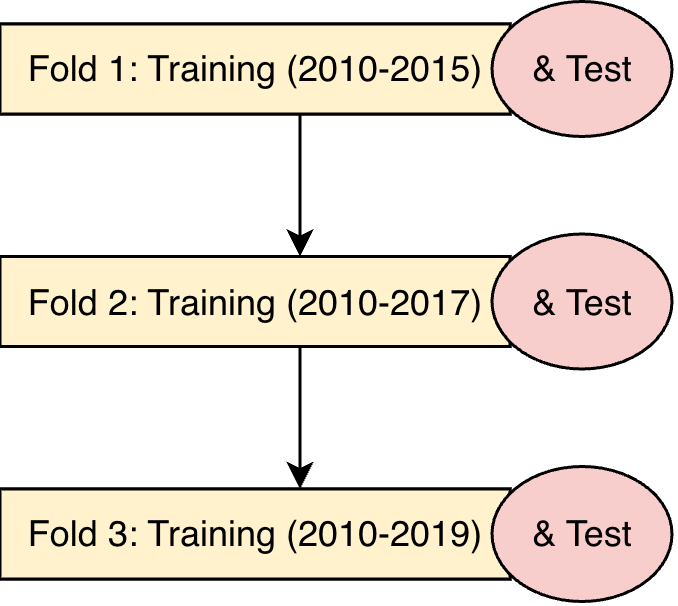
\includegraphics[width=0.3\textwidth]{images/skema_validasi.png}
  \caption{Visualisasi Pembagian Data pada Skema TimeSeriesSplit}
  \label{gambar:skema_validasi}
\end{figure}

Sebagai langkah penanganan atas permasalahan validasi tersebut, dirancang sebuah skema \textit{TimeSeriesSplit} yang beroperasi menggunakan pendekatan rantaian maju (\textit{Forward Chaining}) sebagaimana ditunjukkan pada visualisasi di atas. Skema validasi ini menjaga urutan kronologis data dengan mempartisi set data menjadi $K=5$ lipatan (\textit{folds}) observasi yang berekspansi searah berjalannya waktu. Secara operasional, batas jendela observasi untuk himpunan data latih akan membesar seiring berjalannya putaran lipatan eksperimen, sementara panjang rentang waktu yang digunakan sebagai basis evaluasi pada himpunan data uji dipertahankan konstan.

Desain skema ini digunakan untuk memastikan bahwa algoritma diuji kemampuannya dalam merekonstruksi proyeksi data yang belum pernah dilalui pada fase pembelajaran. Pemisahan dimensi historis dan periode evaluasi bertujuan untuk menguji ketahanan model ketika dihadapkan pada fluktuasi rill kualitas udara di lapangan. Rincian pembagian batas ekspansi observasi kronologis dari kelima lipatan iterasi tersebut dijabarkan sebagai berikut:

\begin{enumerate}
    \item[(a)] {Lipatan 1 (\textit{Fold 1}):} Data latih menggunakan riwayat observasi dari titik mula hingga titik potong $T_1$, dengan pengujian performa prediksi dilakukan pada rentang interval menuju titik $T_2$.
    \item[(b)] {Lipatan 2 (\textit{Fold 2}):} Batas matriks data latih diperluas secara kronologis hingga menyentuh titik potong $T_2$, untuk kemudian dievaluasi pada rentang interval $T_2$ menuju $T_3$.
    \item[(c)] {Lipatan 3 (\textit{Fold 3}):} Komputasi model mengekstraksi riwayat data masa lampau hingga mencapai batas titik $T_3$, yang ditujukan untuk memetakan proyeksi performa pada periode $T_3$ menuju $T_4$.
    \item[(d)] {Lipatan 4 (\textit{Fold 4}):} Dimensi observasi pelatihan berlanjut mengekspansi data latih hingga titik $T_4$, di mana karakteristik model divalidasi untuk cakupan prediksi $T_4$ menuju $T_5$.
    \item[(e)] {Lipatan 5 (\textit{Fold 5}):} Fase final pembelajaran menggunakan dimensi ruang data historis yang paling besar hingga titik batas $T_5$, dengan target evaluasi observasi akhir di tahun 2025.
\end{enumerate}

\section{Desain Modul Penjelasan Model dan Output Pelaporan}

Penerapan pemodelan komputasi berbasis \textit{machine learning} dalam ranah kebijakan publik, khususnya pemantauan lingkungan, memiliki batasan jika beroperasi sebagai sistem yang tertutup (\textit{black-box}). Pemangku kepentingan memerlukan rasionalitas dan transparansi di balik setiap angka prediksi yang dikeluarkan oleh algoritma guna memvalidasi informasi sebelum intervensi dilakukan. Oleh karena itu, perancangan sistem ini mengintegrasikan lapisan interpretasi untuk memberikan justifikasi ilmiah terhadap fluktuasi konsentrasi PM\textsubscript{10} di Jakarta.

Perancangan modul penjelasan ini bertujuan untuk menghubungkan antara kompleksitas matematis model hibrida dengan kebutuhan praktis analis di instansi terkait. Dengan adanya komponen penjelasan model (XAI), sistem menyediakan informasi variabel prediktor tambahan yang memengaruhi perubahan nilai kualitas udara. Hal ini dilakukan untuk memastikan bahwa model menghasilkan karakteristik yang logis secara teori sains atmosfer.

Struktur keluaran pelaporan dirancang untuk menyederhanakan hasil analitik menjadi informasi yang deskriptif dan mudah dipahami oleh pengambil keputusan. Lapisan pelaporan ini merupakan tahap akhir dari seluruh \textit{pipeline} inferensi berkala yang menyatukan hasil prediksi numerik dengan visualisasi atribusi fitur. Dengan demikian, sistem usulan ini dikembangkan sebagai instrumen pendukung keputusan yang transparan.

\subsection{Integrasi \textit{TreeSHAP} pada \textit{Pipeline} Inferensi}

Modul penjelasan model dalam penelitian ini dirancang menggunakan algoritma \textit{TreeSHAP} yang diintegrasikan setelah model \textit{Random Forest} Regresi menyelesaikan proses prediksi non-linier. Pemilihan \textit{TreeSHAP} didasarkan pada efisiensi komputasionalnya dalam menangani model berbasis pohon dan kemampuannya dalam memberikan estimasi nilai Shapley yang konsisten. Secara matematis, interpretasi ini didasarkan pada kontribusi aditif fitur terhadap nilai prediksi rata-rata, sebagaimana dirumuskan pada Persamaan \ref{eq:shap_val}.

\begin{equation}
f(x) = \phi_0 + \sum_{i=1}^{M} \phi_i
\label{eq:shap_val}
\end{equation}
\eqcaption{Formulasi Nilai Prediksi sebagai Penjumlahan Kontribusi Fitur (SHAP)}

Sistem dirancang untuk mengekstraksi nilai Shapley guna menganalisis kontribusi fitur yang memengaruhi kenaikan atau penurunan konsentrasi PM\textsubscript{10}. Penjelasan ini bekerja dengan cara membandingkan hasil prediksi saat suatu fitur hadir dibandingkan dengan saat fitur tersebut absen, sehingga didapatkan bobot pengaruh yang proporsional. Melalui integrasi ini, setiap luaran prediksi harian akan disertai dengan rincian fitur penggerak yang memperkuat hasil pemodelan hibrida.

Dalam implementasinya, modul interpretasi ini dikonfigurasi untuk menghasilkan dua level penjelasan analitik guna memenuhi kebutuhan evaluasi yang berbeda. Level pertama berfokus pada analisis makro untuk melihat pola polusi secara keseluruhan, sedangkan level kedua berfokus pada analisis mikro untuk kasus prediksi harian yang bersifat spesifik. Rincian fungsionalitas dari kedua level penjelasan tersebut dijabarkan sebagai berikut:

\begin{enumerate}
    \item[(a)] {Penjelasan Global (\textit{Summary Plot}):} Tahap ini mengagregasi nilai SHAP dari seluruh data pengujian untuk memetakan hierarki kepentingan fitur secara global. Analisis ini ditujukan untuk memperlihatkan variabel makro, seperti interaksi fotokimiawi $CO \times O_3$ atau variabel \texttt{pm10\_lag1}, yang secara konsisten berkontribusi terhadap fluktuasi polusi udara di wilayah Jakarta.
    \item[(b)] {Penjelasan Local (\textit{Force Plot}):} Tahap ini diaktifkan secara spesifik pada mode inferensi harian untuk membedah prediksi pada tanggal tertentu. Modul ini menghitung vektor kontribusi fitur pada hari $t$ untuk menyediakan alasan logis di balik proyeksi sistem, misalnya mengidentifikasi apakah fluktuasi polusi disebabkan oleh akumulasi polutan sisa hari ini atau akibat variasi cuaca lokal.
\end{enumerate}

\subsection{Desain Laporan Prediksi Harian (\textit{Output Mockup})}

Luaran akhir dari keseluruhan komputasi arsitektur hibrida ini dirancang untuk disajikan dalam sebuah format laporan terpadu yang informatif bagi otoritas terkait. Rancang bangun struktur informasi (\textit{wireframe}) pelaporan harian disusun untuk menyajikan data secara hierarkis, mulai dari indikator utama hingga penjelasan teknis. Hal ini memastikan bahwa pengguna dapat menganalisis poin utama prediksi secara efisien tanpa kehilangan konteks analitiknya.

Penyajian laporan dirancang agar dapat diakses melalui dasbor yang menampilkan visualisasi interaktif dari hasil kalkulasi XAI. Penekanan utama pada visualisasi ini adalah penggunaan elemen warna untuk membedakan faktor pendorong dan faktor pereduksi polusi, sehingga memudahkan proses pemantauan secara intuitif. Dengan desain ini, laporan harian tidak hanya bersifat informatif tetapi juga berfungsi sebagai alat bantu pemantauan terhadap potensi risiko kualitas udara masyarakat.

Struktur informasi dalam pelaporan harian ini terdiri atas tiga panel utama yang bekerja secara sinergis untuk memberikan gambaran kualitas udara. Setiap panel memiliki fungsi spesifik dalam menyampaikan dimensi data kepada pemangku kepentingan. Rincian isi dari ketiga panel utama tersebut didefinisikan sebagai berikut:

\begin{enumerate}
    \item[(a)] {Panel Status Prediksi:} Panel ini menampilkan proyeksi nilai numerik konsentrasi PM\textsubscript{10} untuk satu hari ke depan beserta ambang batas galatnya. Informasi ini kemudian dikonversikan secara otomatis ke dalam kategori Indeks Standar Pencemar Udara (ISPU) sesuai regulasi yang berlaku, seperti kategori "Sedang" atau "Tidak Sehat".
    \item[(b)] {Panel Dekomposisi Kausalitas:} Panel ini memuat visualisasi \textit{SHAP Force Plot} yang memberikan rincian kekuatan pendorong polusi pada hari tersebut. Warna merah digunakan untuk mengindikasikan fitur yang berkontribusi menaikkan tingkat polusi, sedangkan warna biru digunakan untuk merepresentasikan fitur yang memiliki efek mereduksi konsentrasi polutan.
    \item[(c)] {Panel Rekomendasi Preskriptif:} Panel ini menyajikan kesimpulan tekstual yang diturunkan secara otomatis dari hasil analisis modul XAI. Luaran pada panel ini berfungsi sebagai draf informasi penentuan intervensi kebijakan, seperti menyampaikan anjuran pengelolaan mobilitas jika fluktuasi nilai diprediksi akibat akumulasi polutan sisa yang terperangkap oleh kondisi atmosfer yang stabil.
\end{enumerate}